\documentclass[12pt]{beamer}
\setbeamertemplate{navigation symbols}{}
\usetheme{Copenhagen}
\usepackage{listings}
\usepackage{xcolor}
\usepackage{graphicx}
\usepackage{hyperref}
\usepackage{multicol}
\graphicspath{ {imagenes/} }

\definecolor{codegreen}{rgb}{0,0.6,0}
\definecolor{codegray}{rgb}{0.5,0.5,0.5}
\definecolor{codepurple}{rgb}{0.58,0,0.82}
\definecolor{backcolour}{rgb}{0.95,0.95,0.92}

\lstdefinestyle{mystyle}{
    language=c++,
    backgroundcolor=\color{backcolour},   
    commentstyle=\color{codegreen},
    keywordstyle=\color{magenta},
    numberstyle=\tiny\color{codegray},
    stringstyle=\color{codepurple},
    basicstyle=\ttfamily\footnotesize,
    breakatwhitespace=false,         
    breaklines=true,                 
    captionpos=b,                    
    keepspaces=true,                 
    numbers=left,                    
    numbersep=5pt,                  
    showspaces=false,                
    showstringspaces=false,
    showtabs=false,                  
    tabsize=2
}

\lstset{style=mystyle}

\title{Complejidad}
\subtitle{Big O notation}
\author{Tomás Peiretti}
\date{}

\begin{document}

\maketitle

\begin{frame}{Complejidad temporal}
    La \alert{complejidad temporal} permite estimar cuánto tiempo utilizará un algoritmo para una determinada entrada. La idea es representar la \alert{eficiencia} como una función cuyo parámetro sea el tamaño de la entrada. \\
    \medskip
    De esta manera, al calcular la complejidad temporal es posible \alert{saber si un algorimo es lo suficientemente rápido} sin tener que implementarlo. \\
    \medskip
    La complejidad temporal se denota \alert{O(...)} donde los tres puntos representan alguna función.
\end{frame}

\begin{frame}[fragile]{Complejidad temporal: orden de magnitud}
    La complejidad temporal no nos dice cual es el numero exacto de veces que nuestro código se ejecutará, solo representa el orden de magnitud. \\
    \medskip
    \begin{columns}
        \column{0.5\textwidth}Por ejemplo, en los siguientes bucles el código se ejecuta \textbf{3n}, \textbf{n+5} y \textbf{n/2} veces respectivamente, pero la complejidad de cada uno sigue siendo \alert{O(n)}.
        \column{0.4\textwidth}\begin{lstlisting}[basicstyle=\tiny]
for (int i=0; i<3*n; i++)  {
    // .....
} 

for (int i=0; i<n+5; i++)  {
    // .....
}

for (int i=0; i<n; i+=2)  {
    // .....
}
\end{lstlisting}
    \end{columns}
\end{frame}

\begin{frame}[fragile]{Complejidad temporal: orden de magnitud}
    \begin{columns}
        \column{0.9\textwidth}¿Qué complejidad tiene la siguiente función?
        \column{0.1\textwidth}
\includegraphics[width=\textwidth]{thinking_meme.png}
    \end{columns}
\begin{lstlisting}
int sumaTriangular(int m[][1000], int n) {
    int sum=0;
    for(int i=0; i<n; i++) {
        for (int j=i; j<n; j++) {
            sum+=m[i][j];
        }
    }
    return sum;
}
\end{lstlisting}
\end{frame}

\begin{frame}[fragile]{Complejidad temporal: orden de magnitud}
    \centering ¿Qué complejidad tiene la siguiente función? O(\alert{$n^2$})\\
    \medskip
\begin{lstlisting}
int sumaTriangular(int m[][1000], int n) {
    int sum=0;
    for(int i=0; i<n; i++) {
        for (int j=i; j<n; j++) {
            sum+=m[i][j];
        }
    }
    return sum;
}
\end{lstlisting}
\end{frame}

\begin{frame}[fragile]{Complejidad temporal: fases}
    Cuando un algoritmo consiste de múltiples fases (partes, funciones, etc), su complejidad será la complejidad de la \alert{fase que que requiere más tiempo}. \\
    Esto se debe a que la fase que requiere más tiempo (la de mayor complejidad) termina siendo el "cuello de botella" del algoritmo. \\
    \medskip
    \begin{columns}
        \column{0.5\textwidth}Por ejemplo, la siguiente función consiste de tres fases cuya complejidad es \\ O(n + $n^2$ + 1), por lo que su complejidad resultará de O($n^2$).
        \column{0.4\textwidth}\begin{lstlisting}[basicstyle=\tiny]
void miFunc(int & n) {
    for (int i=0; i<n; i++)  {
        // .....
    } 
    
    for (int i=0; i<n; i++)  {
        for (int j=0; j<n; j++)
            // .....
    }
    
    n = -100;
}
\end{lstlisting}
    \end{columns}
\end{frame}

\begin{frame}[fragile]{Complejidad temporal: múltiples variables}
    A veces, la complejidad del algoritmo depende de múltiples factores. Para estos casos, la función tendrá múltiples variables. \\
    \medskip
    Por ejemplo, si debemos recorrer una matriz de N filas y M columnas la complejidad será O(\alert{N*M})
\begin{lstlisting}[basicstyle=\scriptsize]
void imprimeMatriz(int mat[][1000], int n, int m) {
    for (int i=0; i<n; i++)  {
        for (int j=0; j<n; j++)
            cout << mat[i][j] << " ";
        cout << endl;
    }
}
\end{lstlisting}
\end{frame}

\begin{frame}[fragile]{Complejidad temporal}
    \centering ¿Qué complejidad tiene el siguiente programa? \\
    \medskip
\begin{lstlisting}[basicstyle=\tiny]
int sumaFila(int m[][1000], int fila, int tl) {
    int sum=0;
    for(int i=0; i<tl; i++) {
        sum+=m[fila][i];
    }
    return sum;
}

void imprimeMediaMatriz(int mat[][1000], int n, int m) {
    for (int i=0; i<n; i++)  {
        for (int j=0; j<m/2; j++)
            cout << mat[i][j] << " ";
        cout << endl;
    }
}

int main() {

    int mat[2000][1000];
    int n=100, m=50;
    
    imprimeMediaMatriz(mat, n, m);
    cout << sumaFila(mat, 0, m) + sumaFila(mat, n-1, m) << endl;
}
\end{lstlisting}
\end{frame}

\begin{frame}[fragile]{Complejidad temporal}
    \centering ¿Qué complejidad tiene el siguiente programa? O(\alert{N*M}) \\
    \medskip
\begin{lstlisting}[basicstyle=\tiny]
int sumaFila(int m[][1000], int fila, int tl) {
    int sum=0;
    for(int i=0; i<tl; i++) {
        sum+=m[fila][i];
    }
    return sum;
}

void imprimeMediaMatriz(int mat[][1000], int n, int m) {
    for (int i=0; i<n; i++)  {
        for (int j=0; j<m/2; j++)
            cout << mat[i][j] << " ";
        cout << endl;
    }
}

int main() {

    int mat[2000][1000];
    int n=100, m=50;
    
    imprimeMediaMatriz(mat, n, m);
    cout << sumaFila(mat, 0, m) + sumaFila(mat, n-1, m) << endl;
}
\end{lstlisting}
\end{frame}

\begin{frame}[fragile]{Complejidad temporal de funciones recursivas}
    La complejidad de una función recursiva se calcula como el producto entre el número de veces que la función se llama a sí misma y de la complejidad de una única llamada. \\
    \medskip
    Por ejemplo, para la función que obtiene en n-ésimo término de la sucesión de fibonacci:
\begin{lstlisting}
int fibonacci(int n) {
    if (n == 1 || n == 2)
        return 1;
    return fibonacci(n-1) + fibonacci(n-2);
}        
\end{lstlisting}
La llamada fibonacci(n) producirá $2^n$ llamadas y la complejidad de cada llamada será O(\alert{1}), por lo que la complejidad resultante será de O(\alert{$2^n$})
\end{frame}

\begin{frame}[fragile]{Complejidad temporal de funciones recursivas}
    \begin{columns}
        \column{0.5\textwidth}¿Qué complejidad tiene la siguiente función recursiva?
        \column{0.2\textwidth}
\includegraphics[width=\textwidth]{thinking_meme2.jpg}
    \end{columns}
\begin{lstlisting}
void imprimirALoLoco(int arr[], int n) {

    if (n < 0) return;

    for (int i=0; i<n; i++) {
        cout << arr[i] << " ";
    }
    cout << endl;

    imprimirALoLoco(arr, n-1);
}
\end{lstlisting}
\end{frame}

\begin{frame}[fragile]{Complejidad temporal de funciones recursivas}
    \centering ¿Qué complejidad tiene la siguiente funcion? O(\alert{$n^2$}) \\
    \medskip
\begin{lstlisting}
void imprimirALoLoco(int arr[], int n) {
    
    if (n < 0) return;

    for (int i=0; i<n; i++) {
        cout << arr[i] << " ";
    }
    cout << endl;

    imprimirALoLoco(arr, n-1);
}
\end{lstlisting}
\end{frame}

\begin{frame}{Complejidades más usuales}
    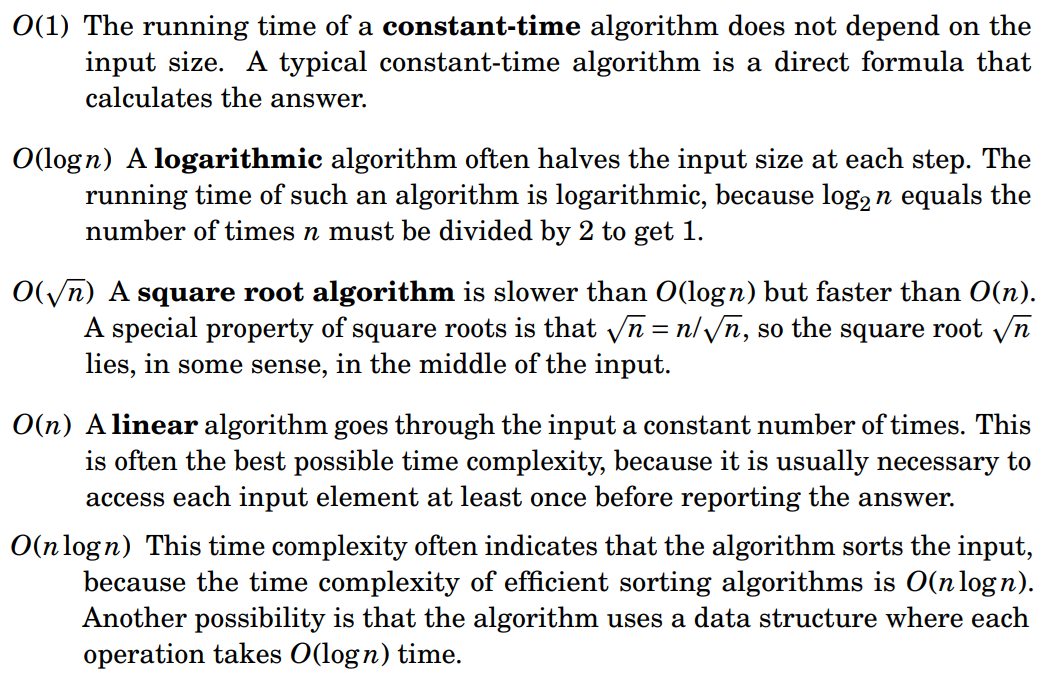
\includegraphics[width=\textwidth]{complejidades1.png}
    \centering\url{https://github.com/pllk/cphb/blob/master/book.pdf}
\end{frame}

\begin{frame}{Complejidades más usuales}
    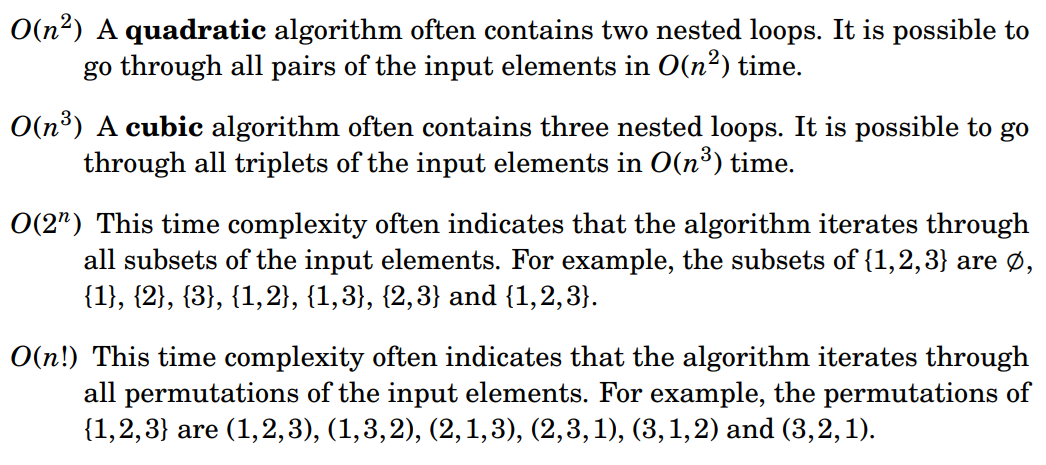
\includegraphics[width=\textwidth]{complejidades2.png}
    \centering\url{https://github.com/pllk/cphb/blob/master/book.pdf}
\end{frame}

\end{document}